\chapter{Experimental Setup and Results}\label{ch:results}
***************************************\\
Benchmark can be a simple control design \\
Benchmark can be Praveen's MPC controller to compare results \\
Benchmark can be open loop response Figure \ref{fig:QROL}.
\begin{figure}[h!]
	\centering
	\makebox[\textwidth][c]{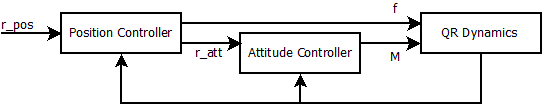
\includegraphics[width=.2\paperwidth]{./StyleStuff/QRloop.png}}
	\caption{Open Loop control QR \label{fig:QROL}}
\end{figure}
***************************************\\

\section{Software}
Simulink
Solvers etc.

\section{Experiments}
\subsection{Performance Criteria}
***************************************\\
Performance that can be evaluated for the cases in Figure \ref{fig:routes}. Performance can be specified as the following items.
\begin{outline}
	\1 Step Response
	\2 Settling time (if swing minimization is important)
	\2 Rising time (important if time critical)
	\2 Overshoot (if max swing is critical)
	\2 Steady state error / swing of load (if accuracy is important)
	
	\1 Disturbance Rejection
	
	\1 Trajectory tracking
	\2 Can we minimize time, while minimizing position error (All Cases)
	\2 Minimum position error (All Cases)
	\2 Maximum amplitude/frequency of wave with respect to stability (Case B)
	
	\1 Computational Effort (?)
\end{outline}

Explain cases, why interesting and what can be expected?\\

\subsection{Case A}
\subsection{Case B}
\subsection{Case C}

\begin{figure}[h!]
	\centering
	\makebox[\textwidth][c]{\includegraphics[width=.2\paperwidth]{./StyleStuff/routes.png}}
	\caption{Cases of which the performance could be evaluated \label{fig:routes}}
\end{figure}

\section{Command Filtering}
To compute $ \dot{R}_c, \ddot{R}_c,\dot{q}_c, \ddot{q}_c $, the virtual control command to stabilize the loop within. \cite{Farrell2009}

\begin{align}\label{eq:CF}
\frac{x_c}{x_c^o}&=\frac{\omega_{n1}}{s+\omega_{n1}}\cdot\frac{\omega_{n2}^2}{s^2+2\zeta\omega_{n2}s+\omega_{n2}^2}\\
\Rightarrow x_c^{'''}&=-(2\zeta\omega_{n2}+\omega_{n1})x_c^{''}-(2\zeta\omega_{n1}\omega_{n2}+\omega_{n2}^2)x_c^{'}-(\omega_{n1}\omega_{n2} ^2)(x_c-x_c^o)
\end{align}

A command filter is implemented by following examples from \cite{Farrell2008} and \cite{Djapic2008}. The load attitude controller generates a commanded QR attitude $ R_c $ and the load position controller generates a commanded load attitude $ q_c $. The controllers contain functions of these signals and their derivatives. Instead differentiation of these signals, the signals are obtained by integration by filtering the original signals $ R_c^o $ and $ q_c^o $. The state space implementation of this filter is \cite{Djapic2008}
\begin{align}\label{key}
\dot{x}_1 &= x_2\\
\dot{x}_2 &= -2\zeta\omega_nx_2-\omega_n^2(x_1-x_c^o)
\end{align}
where $ x_1 = x_1$ and $ \dot{x}_c = x_2 $. The transfer function has the form
\begin{equation}\label{key}
\frac{X_c(s)}{X_c^o(s)}=H(s)=\frac{\omega_n^2}{s^2+2\zeta\omega_ns+\omega_n^2}
\end{equation}
Where $ x_c $ is the filtered signal, $ \zeta $ the damping ratio and $ \omega_n $ the undamped natural frequency. See Figure \ref{fig:CF}.

\section{Results}
\subsection{Case A}
\subsection{Case B}
\subsection{Case C}


\section{Conclusion}

